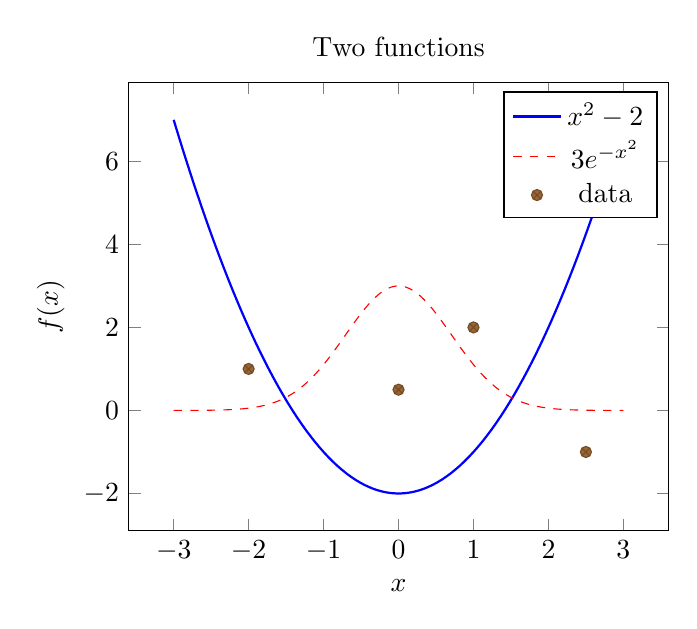
\begin{tikzpicture}
\begin{axis}[xlabel={$x$}, ylabel={$f(x)$}, domain=-3:3, samples=100, title={Two functions}]
  \addplot[blue, thick] {x^2 - 2};
  \addplot[red, dashed] {exp(-x^2) * 3};
  \addplot+[only marks] coordinates {(-2,1) (0,0.5) (1,2) (2.5,-1)};
  \legend{$x^2 - 2$, $3e^{-x^2}$, data}
\end{axis}
\end{tikzpicture}
